\chapter{Operating System Layer: In-Network Memory Management}
\label{chap:os}
In the previous chapter, we explored the design of memory management for disaggregated architectures at the service layer. Specifically, we examined how serverless applications, which are inherently aware of disaggregated memory and compute resources, require explicit memory management for handling intermediate data. Integrating such applications with \jiffy is straightforward, as they can directly benefit from \jiffy's elasticity and lifetime management features. However, general-purpose applications (beyond serverless data analytics) are typically developed without any knowledge of the underlying hardware specifics, such as disaggregated resources. As a result, integrating these applications with external memory services (e.g., \jiffy) often necessitates significant code modifications to accommodate their APIs, which may present an undesirable burden for developers.

In traditional monolithic architectures, memory management is typically handled by the operating system (OS), which manages virtual and physical pages, performs memory address translation, enforces memory protection, and provides a simple interface to user applications. This abstraction hides the hardware details, thereby easing the burden of memory management for developers. If the OS is made aware of disaggregated architectures and can transparently manage memory, it would be possible to migrate existing applications to these architectures without requiring any code modifications. 

The fundamental distinction between performing memory management at the OS layer versus the service layer lies in the scope and specificity of the functionality provided. The OS must offer highly general functionality that applies to all applications, while the service layer can afford to provide more specialized features tailored to specific application types (e.g., lifetime management in \jiffy). A key question that arises is where the OS should be situated within the disaggregated architecture. Unlike monolithic architectures, where the OS resides directly on each server, disaggregated architectures lack a single, centralized server. We observe that the network interconnect (e.g., Ethernet) presents a promising point for implementing OS-level memory management (\ref{sec:mindbackground}). However, even if memory management functionalities are implemented transparently within the OS, their performance may vary depending on the application type due to fundamental differences in how resources are organized (\ref{sec:needforpulse}).

In this chapter, we shift our focus to embedding memory management functionality directly within the OS. We first introduce \mind, an in-network OS design that enables transparent memory management for disaggregated resources. Following this, we present \pulse, an in-network near-memory accelerator designed to optimize performance for pointer traversal workloads.


\section{Background: MIND}
\label{sec:mindbackground}




Implementing memory management at the OS layer in disaggregated architectures poses three significant challenges. First, remote memory access requires low latency and high throughput, with targets of $10~\mu$s latency and $100$ Gbps bandwidth per compute blade~\cite{legoos, infiniswap, fastswap, disagg}. Second, both compute and memory resources must scale elastically to meet varying workloads. Finally, widespread adoption of disaggregated memory necessitates support for unmodified applications, minimizing the need for developers to rewrite code.

We introduce \mind, the first memory management system designed for rack-scale disaggregated memory, addressing these challenges by embedding the memory management module (\mmm) directly within the network fabric and leveraging programmable network switches~\cite{progswitch1, progswitch2}.

The placement of \mind's memory management \textit{within the network fabric} is motivated by three key factors: (1) its central location provides a global view of the system, enabling direct memory access without requiring metadata coherence, (2) virtual memory access bears a structural similarity to network address access~\ref{table:isomorph}, and programmable network switches~\cite{progswitch1} are capable of executing at line rate, making them suitable for implementing memory management logic, and (3) incorporating cache coherence logic into the network fabric helps reduce latency and bandwidth overhead.

\begin{table}
    \caption[Parallels between memory \& networking primitives]{\small \textbf{Parallels between memory \& networking primitives.}}
    \label{table:isomorph}
    \centering
    \scriptsize
    \renewcommand{\arraystretch}{1.2}
    \begin{tabular}{p{3cm} p{1cm}p{3cm}}
      \hline
      \textbf{Virtual Memory} &$\Longleftrightarrow$ &\textbf{Networking} \\\hline\hline
      Memory allocation&&IP assignment\\
      Address translation &&IP forwarding\\
      Memory protection  &&Access control\\
      Cache invalidations &&Multicast\\
      \hline
    \end{tabular}
\end{table}

\mind provides a \textit{transparent virtual memory} abstraction to applications, functioning similarly to traditional OS mechanisms. It intercepts memory allocations on CPU blades and performs memory operations via RDMA, using a switch-based MMU for managing cache coherence. Memory blades store pages and directly handle RDMA requests, enabling true hardware disaggregation. 

\begin{figure*}[!t]
\centering
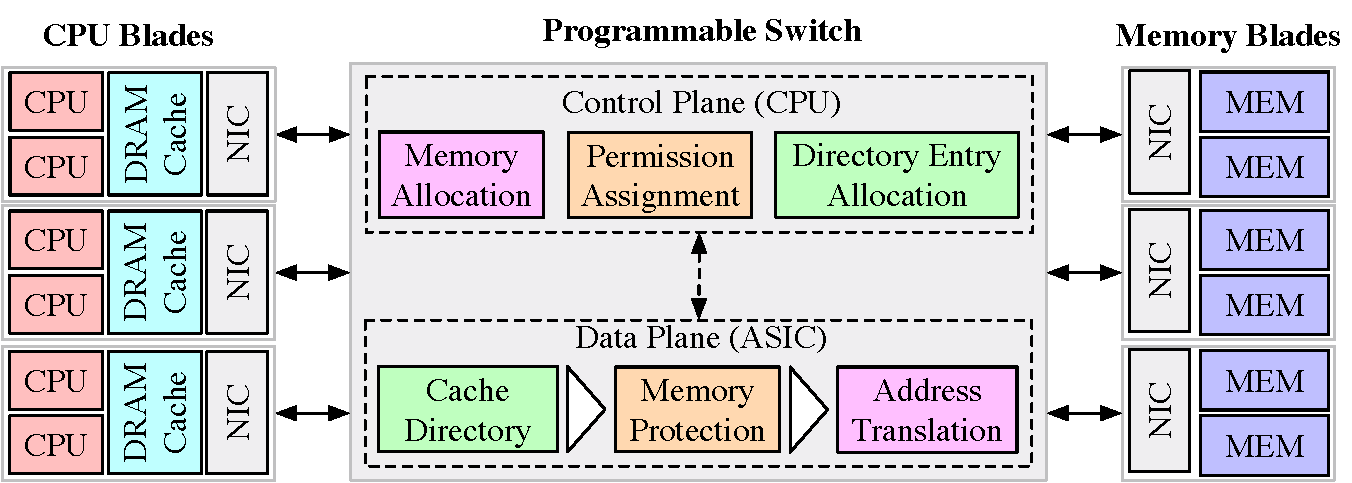
\includegraphics[width=0.55\textwidth]{fig/mind/design}\hspace{3em}
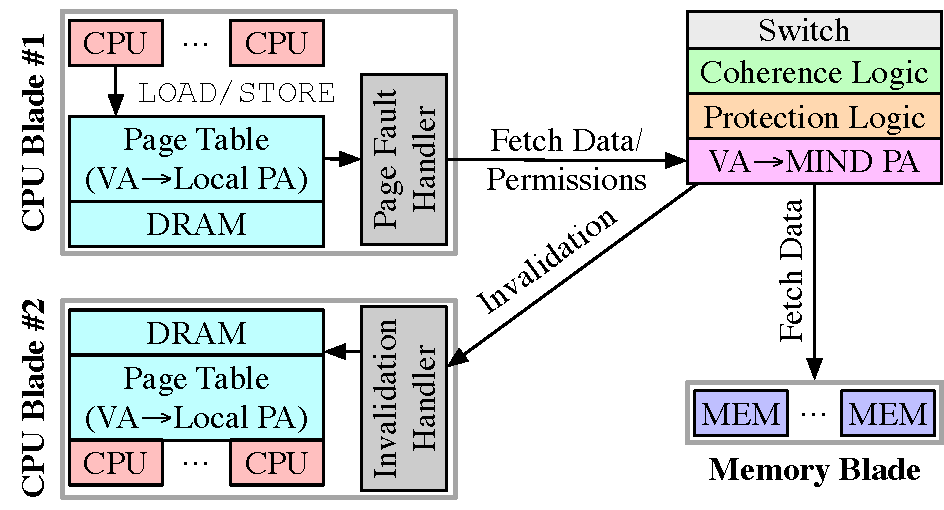
\includegraphics[width=0.35\textwidth]{fig/mind/data_flow}%\vspace{-1em}
\vspace{-0.5em}
\caption[High-level \mind architecture and data flow for memory accesses in \mind]{\textbf{(left) High-level \mind architecture, and, (right) data flow for memory accesses in \mind.}}
\label{fig:system_diagram}
\end{figure*}

Figure~\ref{fig:system_diagram}(left) presents an overview of \mind's design, while Figure~\ref{fig:system_diagram}(right) illustrates its memory access flow. CPU blades run user processes and utilize local DRAM as a cache. Memory allocations and deallocations are intercepted and forwarded to the switch control plane, which manages memory allocation and access permissions. All memory operations are handled by the CPU cache, with virtual addresses translated locally. If a requested page is not cached, a page fault triggers an RDMA request to fetch it from the memory blades. Coherence updates may also trigger page faults, which are handled by the switch. 

Since CPU blades do not maintain memory metadata, RDMA requests operate solely on virtual addresses. The switch's data plane intercepts these requests, managing cache coherence, permission verification, and address translation. If no cache contains the requested page, the switch forwards the request to the appropriate memory blade. \mind relies on one-sided RDMA, removing the need for CPUs on memory blades and paving the way for complete hardware disaggregation.


